\chapter{Requirement Analysis}
\label{chap:requirement-analysis}

\section{Stakeholder Analysis}
\label{section:stakeholder-analysis}

Stakeholders are individuals, groups, or entities that have an interest,
concern, or stake in a particular project, decision, organization, or
system. The following stakeholders have been identified for FigureFlow,
with a primary focus on viewers and broadcasters rather than technical
or officiating roles.

\begin{itemize}
    \item \textbf{Casual Viewers} are the primary target audience.
    These are Olympic and figure skating fans who watch competitions
    without deep technical knowledge of jump classification. They
    require clear, accessible labels and brief explanations delivered
    in real time.

    \item \textbf{Serious Enthusiasts} are competitive skating followers
    who actively engage with scoring and technical panel decisions.
    They require accurate predictions with confidence scores to support
    informed discussion.

    \item \textbf{Broadcasters} include live commentators and streaming
    platforms that integrate FigureFlow into a broadcast pipeline.
    They require low-latency, reliable jump identification to enhance
    live coverage without introducing errors.

    \item \textbf{Developers} are responsible for building, training,
    and maintaining the recognition pipeline. They require access to
    labeled pose data and evaluation metrics to iterate on the model.
\end{itemize}


\section{User Stories and Use Cases}
\label{section:user-stories-use-cases}

\subsection{User Stories}

User stories are organized by stakeholder group and capture what each
group needs from FigureFlow in the format: \textit{``As a [stakeholder],
I want to [action] so that [benefit].''}

\subsubsection*{Casual Viewer (Primary)}

\begin{itemize}
    \item As a casual Olympics viewer, I want jump names overlaid on
    screen so that I can understand what is being scored during a
    performance.

    \item As a new figure skating fan, I want simple on-screen
    explanations so that I do not need prior skating expertise to
    follow along.
\end{itemize}

\subsubsection*{Serious Enthusiast}

\begin{itemize}
    \item As a competitive skating follower, I want to verify technical
    panel calls using the system's predictions so that I can engage
    in informed discussions about judging decisions.

    \item As an ISU Grand Prix watcher, I want confidence scores
    displayed alongside jump labels so that I can assess how reliable
    each prediction is relative to a human caller.
\end{itemize}

\subsubsection*{Broadcaster}

\begin{itemize}
    \item As a live commentator, I want reliable jump identifications
    that replace manual program sheet lookups so that I can avoid
    mistakes during live broadcasts.

    \item As a streaming platform operator, I want end-to-end latency
    below 100ms so that jump overlays remain synchronized with the
    live video feed.
\end{itemize}


\subsection{Use Cases}

The three user stories below are expanded into use cases at increasing
levels of detail.

\subsubsection*{Brief Use Case: Upload Video}

A user uploads a pre-recorded video file. The system accepts the file,
validates the format, and queues it for processing.

\subsubsection*{Casual Use Case: Display Prediction}

After processing, the user opens the results view. The system presents
the original video with jump labels and confidence scores overlaid at
the corresponding timestamps. The user can pause, scrub, and review
individual jump events. If no jump is detected in a segment, no label
is shown.

\subsubsection*{Fully-Dressed Use Case: Live Jump Identification}

\begin{table}[h]
    \centering
    \renewcommand{\arraystretch}{1.4}
    \caption{Fully-Dressed Use Case: Live Jump Identification}
    \label{tab:usecase-classify}
    \begin{tabular}{|p{3.5cm}|p{9.5cm}|}
        \hline
        \textbf{Use Case Name}
            & Live Jump Identification \\
        \hline
        \textbf{Actors}
            & Casual Viewer, Broadcaster \\
        \hline
        \textbf{Goal}
            & Receive an accurate jump label during a live competition
              broadcast. \\
        \hline
        \textbf{Preconditions}
            & A broadcast video stream is active and the classification
              model is loaded. \\
        \hline
        \textbf{Main Success Scenario}
            & 1. System receives a video frame from the broadcast feed.
              \newline
              2. YOLOv8 detects and tracks the skater within a bounding
              box. \newline
              3. MediaPipe extracts 33 pose keypoints from the detected
              region. \newline
              4. LSTM processes a 100-frame pose sequence and outputs
              a jump label with a confidence score
              (e.g., ``Triple Axel, 87\%''). \newline
              5. Overlay displays the jump name and a brief takeoff
              explanation to the viewer. \\
        \hline
        \textbf{Alternative Flows}
            & 2a. If confidence falls below 70\%, the system suppresses
              the label and displays no prediction for that sequence.
              \newline
              3a. If pose detection fails due to occlusion or motion
              blur, the system skips the affected frame and resumes
              processing on the next available frame. \\
        \hline
        \textbf{Postconditions}
            & Jump name and confidence score are displayed as an overlay
              and optionally logged for post-broadcast review. \\
        \hline
    \end{tabular}
\end{table}


\section{Use Case Diagrams}
\label{section:use-case-diagrams}

\begin{figure}[htbp]
    \centering
    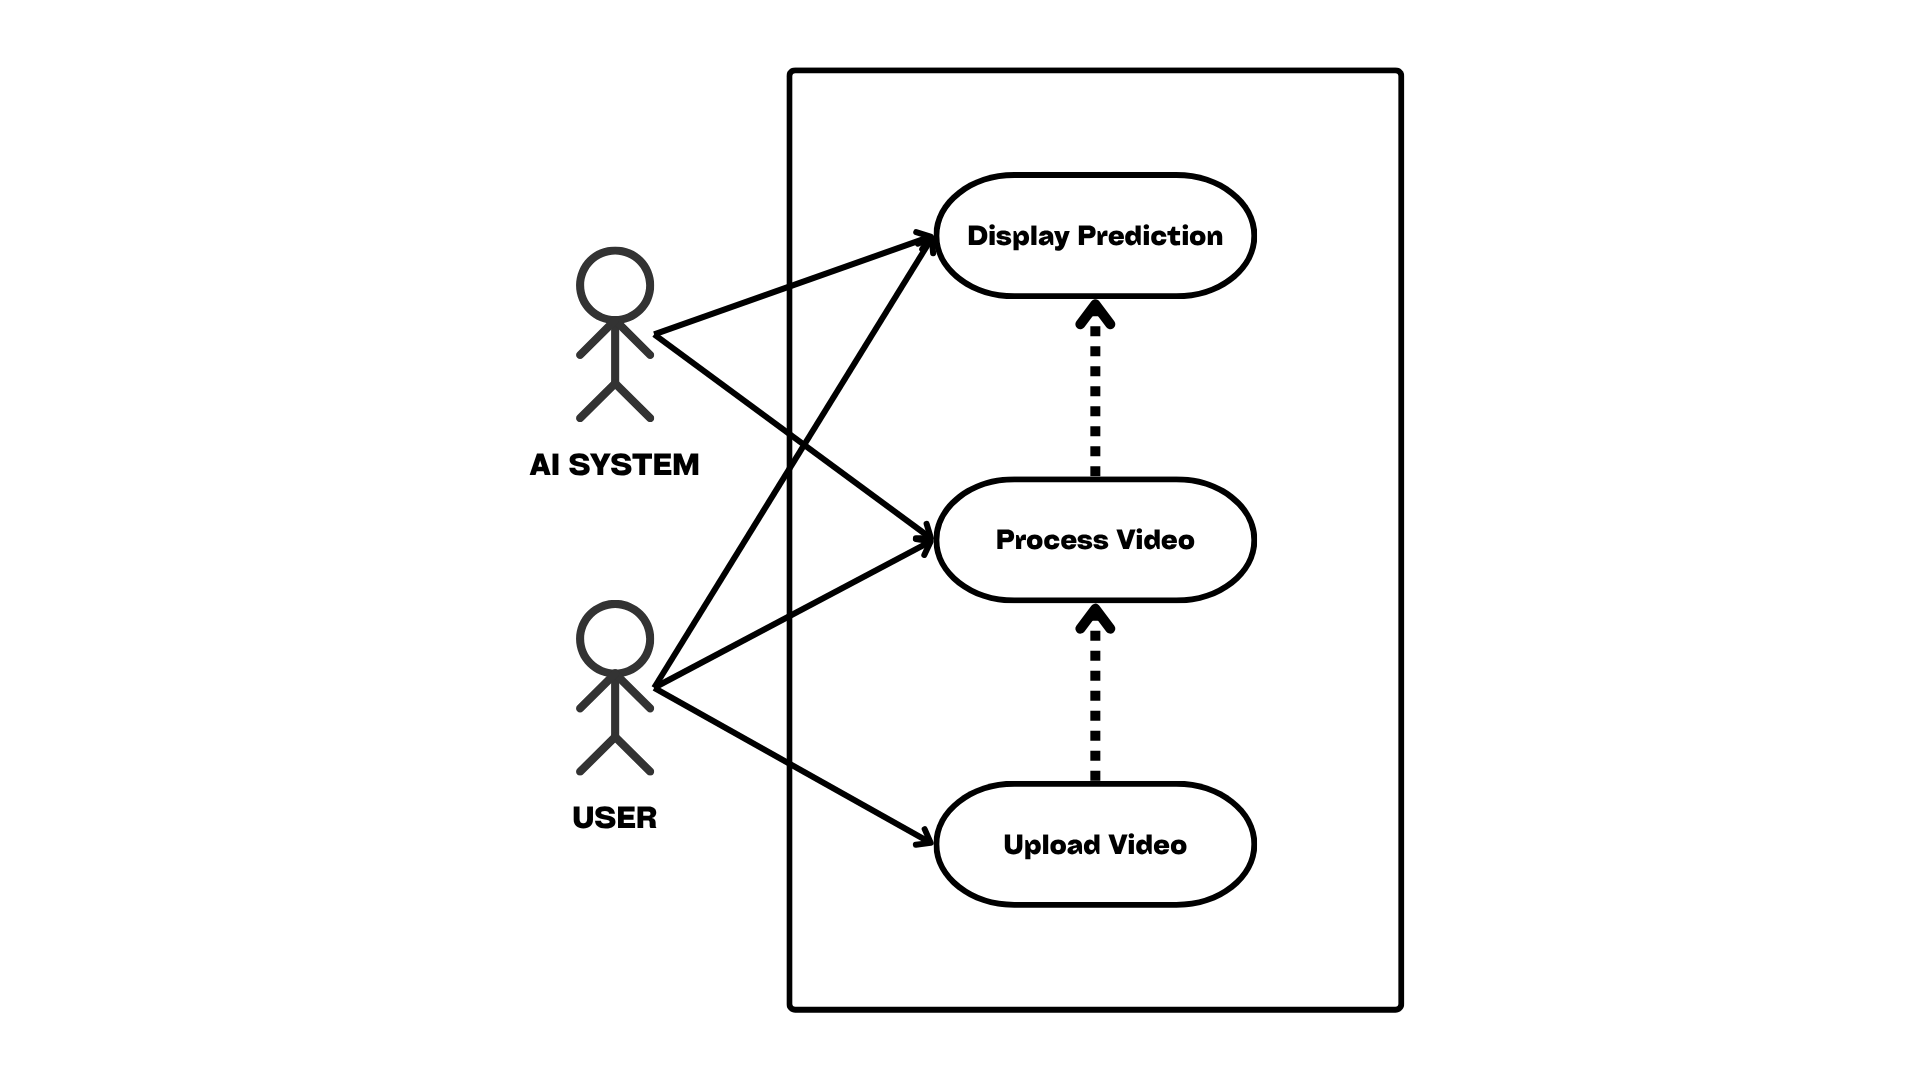
\includegraphics[width=1.1\textwidth, keepaspectratio]{assets/images/usecase-diagram.png}
    \caption{Actors and use cases for FigureFlow}
    \label{fig:usecase}
\end{figure}

Figure~\ref{fig:usecase} illustrates the actors and use cases
for FigureFlow. The two primary actors are the \textbf{User} (covering
casual viewers, serious enthusiasts, and broadcasters) and the
\textbf{System} (the automated AI pipeline).

The three core use cases identified in this diagram are as follows.

\begin{itemize}
    \item \textbf{Upload Video:} the user provides a pre-recorded
    video file as input to the system for offline processing and
    classification.

    \item \textbf{Process Video:} the system applies the detection,
    pose estimation, and LSTM classification pipeline to produce a
    sequence of jump predictions with confidence scores.

    \item \textbf{Display Prediction:} the system renders the
    classified jump label as an overlay on the video and presents a
    summary of results in the dashboard interface.
\end{itemize}


\section{User Interface Design}
\label{section:user-interface-design}

The FigureFlow interface is designed to be minimal and accessible,
prioritising clarity for casual viewers who have no prior skating
expertise. The proposed design consists of three components.

\begin{itemize}
    \item \textbf{Video Player:} a full-width player that streams
    or plays back the input footage with frame-accurate
    synchronization.

    \item \textbf{Jump Label Overlay:} a semi-transparent annotation
    rendered directly on the video frame, displaying the predicted jump
    type (e.g., \textit{Triple Axel}, \textit{Triple Lutz}) alongside
    the confidence score and a one-line plain-language explanation
    (e.g., ``hardest jump, forward takeoff'').

    \item \textbf{Dashboard Panel:} a sidebar or bottom panel
    summarizing all detected jumps, their timestamps, and
    classification results for the full performance, supporting
    post-session review by enthusiasts and broadcasters.
\end{itemize}

\newpage\vspace*{-\topskip}\vspace*{-2cm} 
\begin{figure}[t!]
    \centering
    
\includegraphics[width=0.8\textwidth]{images/axel.png}
    \caption{FigureFlow User Interface Design}
    \label{fig:ui-design}
\end{figure}